\documentclass{standalone}
\usepackage{tikz}
\usetikzlibrary{shapes.geometric, arrows.meta, positioning, fit, calc, backgrounds}

\begin{document}
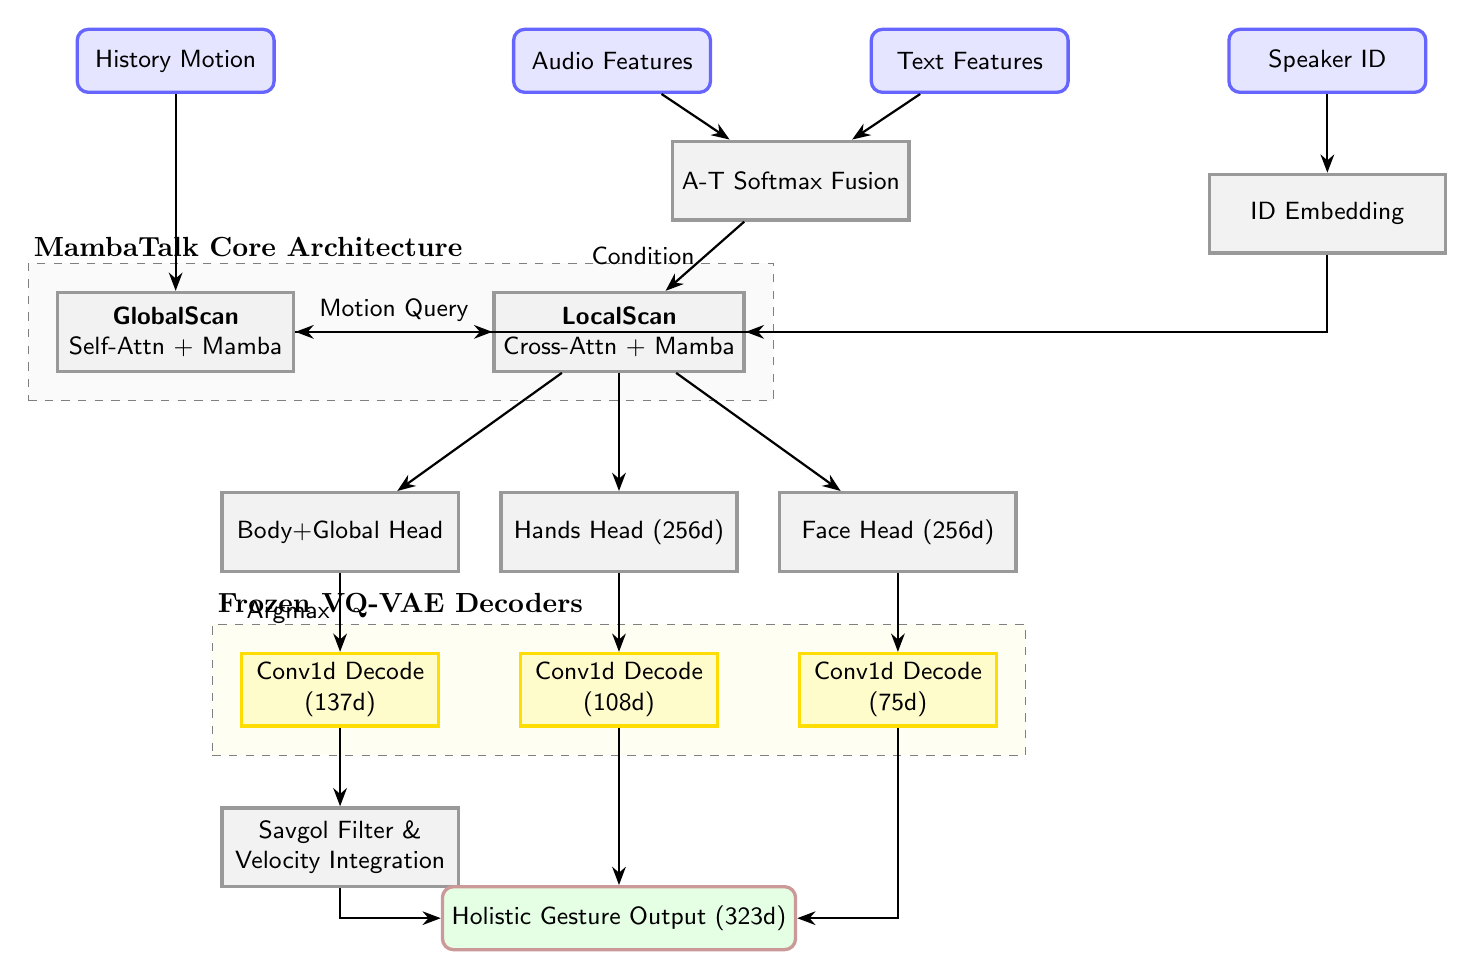
\begin{tikzpicture}[
    >=Stealth,
    node distance=1.5cm and 2cm,
    font=\sffamily\small,
    input/.style={rectangle, draw=blue!60, fill=blue!10, very thick, minimum width=2.5cm, minimum height=0.8cm, align=center, rounded corners},
    module/.style={rectangle, draw=gray!80, fill=gray!10, very thick, minimum width=3cm, minimum height=1cm, align=center},
    vqvae/.style={rectangle, draw=yellow!80!orange, fill=yellow!20, very thick, minimum width=2.5cm, minimum height=0.8cm, align=center},
    output/.style={rectangle, draw=pink!80!black, fill=green!10, very thick, minimum width=4cm, minimum height=0.8cm, align=center, rounded corners},
    group/.style={rectangle, draw=black!50, dashed, inner sep=10pt, fill=black!2}
]

% Inputs
\node[input] (audio) {Audio Features};
\node[input] (text) [right=of audio] {Text Features};
\node[input] (id) [right=of text] {Speaker ID};
\node[input] (motion) [left=of audio, xshift=-1cm] {History Motion};

% Fusion
\node[module] (fusion) [below=1cm of $(audio)!0.5!(text)$] {A-T Softmax Fusion};
\node[module] (idemb) [below=1cm of id] {ID Embedding};
\draw[->, thick] (audio) -- (fusion);
\draw[->, thick] (text) -- (fusion);
\draw[->, thick] (id) -- (idemb);

% Core
\node[module] (global) [below=2.5cm of motion] {\textbf{GlobalScan}\\Self-Attn + Mamba};
\node[module] (local) [right=2.5cm of global] {\textbf{LocalScan}\\Cross-Attn + Mamba};

\draw[->, thick] (motion) -- (global);
\draw[->, thick] (idemb) |- (global);
\draw[->, thick] (global) -- node[above] {Motion Query} (local);
\draw[->, thick] (fusion) -- node[left] {Condition} (local);
\draw[->, thick] (idemb) |- (local);

% Background box for core
\begin{scope}[on background layer]
    \node[group, fit=(global) (local)] (core_box) {};
    \node[anchor=south west, inner sep=2pt, font=\bfseries] at (core_box.north west) {MambaTalk Core Architecture};
\end{scope}

% Classifiers
\node[module] (head_hand) [below=1.5cm of local] {Hands Head (256d)};
\node[module] (head_body) [left=0.5cm of head_hand] {Body+Global Head};
\node[module] (head_face) [right=0.5cm of head_hand] {Face Head (256d)};

\draw[->, thick] (local) -- (head_body);
\draw[->, thick] (local) -- (head_hand);
\draw[->, thick] (local) -- (head_face);

% VQ-VAE
\node[vqvae] (vq_body) [below=1cm of head_body] {Conv1d Decode\\(137d)};
\node[vqvae] (vq_hand) [below=1cm of head_hand] {Conv1d Decode\\(108d)};
\node[vqvae] (vq_face) [below=1cm of head_face] {Conv1d Decode\\(75d)};

\draw[->, thick] (head_body) -- node[left] {Argmax} (vq_body);
\draw[->, thick] (head_hand) -- (vq_hand);
\draw[->, thick] (head_face) -- (vq_face);

% Background box for VQ
\begin{scope}[on background layer]
    \node[group, fill=yellow!5, fit=(vq_body) (vq_hand) (vq_face)] (vq_box) {};
    \node[anchor=south west, inner sep=2pt, font=\bfseries] at (vq_box.north west) {Frozen VQ-VAE Decoders};
\end{scope}

% Post processing
\node[module] (savgol) [below=1cm of vq_body] {Savgol Filter \&\\Velocity Integration};
\draw[->, thick] (vq_body) -- (savgol);

% Output
\node[output] (out) [below=2cm of vq_hand] {Holistic Gesture Output (323d)};
\draw[->, thick] (savgol) |- (out);
\draw[->, thick] (vq_hand) -- (out);
\draw[->, thick] (vq_face) |- (out);

\end{tikzpicture}
\end{document}